In this section, I will propose an approach for clustering areas within the printing plate with anomalous behaviours. With this approach, we should be able to clustering temperature profiles that exhibit a similar behaviour considering also the distance in the printing plane. This algorithm is based on functional data analysis. The analysis of functional data allows us to gain a comprehensive and detailed understanding of the anomalies, which would enable us to discern if there are specific zones on the print plane behaving irregularly and to understand how the hot spot might influence the mechanical properties of the printed part. In section \ref{sec:fda}, I will provide a brief introduction to functional data analysis, in section \ref{sec:bvc}, I will provide a detailed explanation of the Bagging Voronoi algorithm for functional data clustering and in section \ref{sec:bcv-cases} I will present three successful case studies of algorithm application.

% Unsupervised classification >>>
\section{Unsupervised Learning}
\label{sec:clustering}
In this section, I will briefly introduce the concept of unsupervised learning, and specifically clustering. The purpose of this thesis is not to provide a detailed explanation of machine learning algorithms; thus, I will be as concise as possible, giving the readers the essential tools to understand the algorithm I will describe in \ref{sec:bvc} without overwhelming them. 
Before delving into the specifics of clustering, let's examine the distinction between unsupervised and supervised learning. Supervised learning is a machine learning approach defined using labeled datasets. These datasets are designed to train or "supervise" algorithms to classify data or predict outcomes accurately. The model can measure its accuracy and learn over time using labeled inputs and outputs. Unsupervised learning uses machine learning algorithms to analyze and cluster unlabeled data sets. These algorithms discover hidden patterns in data without the need for an apriori human classification. Indeed, unsupervised learning is also defined as "learning without a teacher" in Hastie et al. \cite{tibshirani_elements_2008}. So, the main difference between supervised and unsupervised learning is the data in input: in the first case, data is labeled, while in the second case is not. Clustering is an unsupervised learning technique.
The aim of all clustering algorithms is to organize a collection of entities into subsets or "clusters" wherein elements within a cluster are as similar as possible, whereas data in different clusters are as dissimilar as possible. So, the goal of clustering is to minimize the within-clusters variance while maximizing the between-clusters variance. But how do we define if two observations in the collection are similar? We have to rely on the concept of distance between the two observations. In Fig. \ref{fig:clustering} there is an example of simulated data in the plane clustered into 3 clusters using the K-Means algorithm.
\begin{figure}[H]
    \centering
    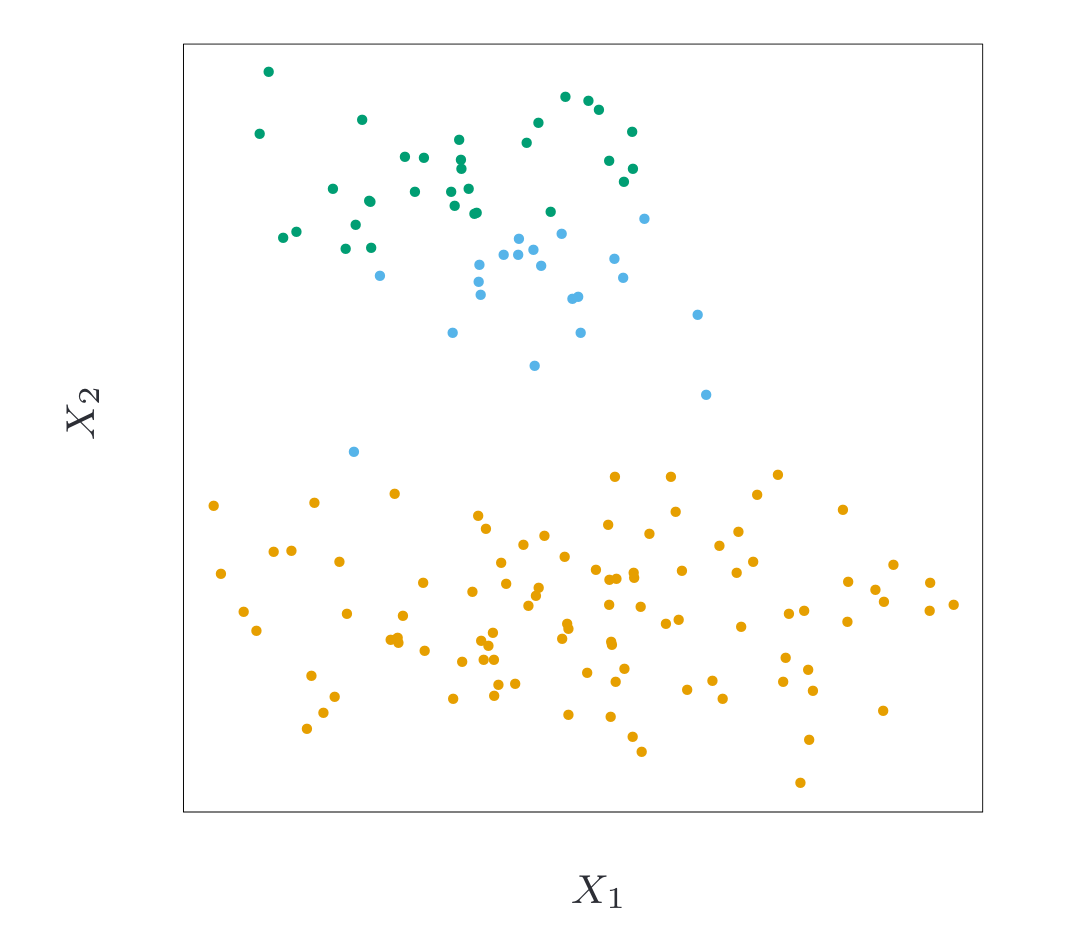
\includegraphics[width=0.5\textwidth]{Images/clustering.png}
    \caption[Example of clustering.]{Simulated data clustered into 3 classes. Adapted from \cite{tibshirani_elements_2008}.}
    \label{fig:clustering}
\end{figure}
There are several different clustering algorithms that can be divided into two main groups, as in \cite{james_introduction_2021}: K-Means clustering and hierarchical clustering. In K-Means clustering, we try to divide observation into a pre-specified number of clusters. On the other hand, in hierarchical clustering, we do not specify the number of clusters in advance, but we rely on the dendrogram, a tree-like visual representation of the observations, that allows us to visualize all the clustering steps. As we will see in section \ref{sec:bvc}, the number $K$ of clusters is an input of the algorithm, making hierarchical clustering not suitable for our purposes. In \ref{subsec:kmeans}, I will describe the K-Means algorithm, the algorithm used in Appendix \ref{ap:Python}. But before delving into the algorithm's description, I also want to explain the concept of bagging for clustering. It is based on the concept of bootstrapping. Bootstrapping is a resampling technique that helps in finding more reliable results from a clustering algorithm. As we will see in the next section, we will perform multiple clustering "rounds" in order to find a frequency distribution of the belongings of the observation to a cluster.
The final cluster label for each observation will be the "most probable correct result" by majority voting.

\subsection{K-Means Clustering Algorithm}
\label{subsec:kmeans}
We begin by defining some notation for describe the K-Means algorithm. Let $C_1,\dots,C_k$ denotes the sets containing all the indices of the observation in respective the respective cluster. K-Means clustering is a very simple clustering algorithm we can use for complete partitioning a data collection of observation $\mathbf{x}=\left(X_1, \dots, X_p \right)$, described by $p$ features, into $K$ distinct, non-overlapping clusters. This means that:
\begin{enumerate}
    \item $C_1 \cup C_2 \cup \dots \cup C_K=\{1,\dots,n\}$. So, each observation belongs to at least one of the $K$ clusters.
    \item $C_k\cap C_{k'}=0$ for all $k\neq k'$. In other words, there is no observation belonging to more than one cluster.
\end{enumerate}

Each observation will be assigned to one cluster and one cluster only. In algorithm \ref{alg:kmeans} there is the description of K-Means clustering algorithm.
\begin{algorithm}
    \caption{K-Means Clustering}
    \label{alg:kmeans}
    \begin{algorithmic}[1]
    \STATE {Initialize the number of cluster $K$.}
    \STATE {Randomly assign a number $1,\dots,K$ to each of the observations. These serve as initial cluster assignments for the observations.}
    \WHILE{clustering assignments is changing}
    \STATE{For each of the $K$ clusters, compute the cluster centroid. The $k$-th cluster centroid is the vector of the $p$ feature means for the observations in the $k$-th cluster.}
    \STATE{Assign each observation to the cluster whose centroid is closest (where closest is defined using Euclidean distance).}
    \ENDWHILE
    \end{algorithmic}
\end{algorithm} 
In Fig. \ref{fig:clustiteration} there is an example of iterations of Algorithm \ref{alg:kmeans}.
\begin{figure}
    \centering
    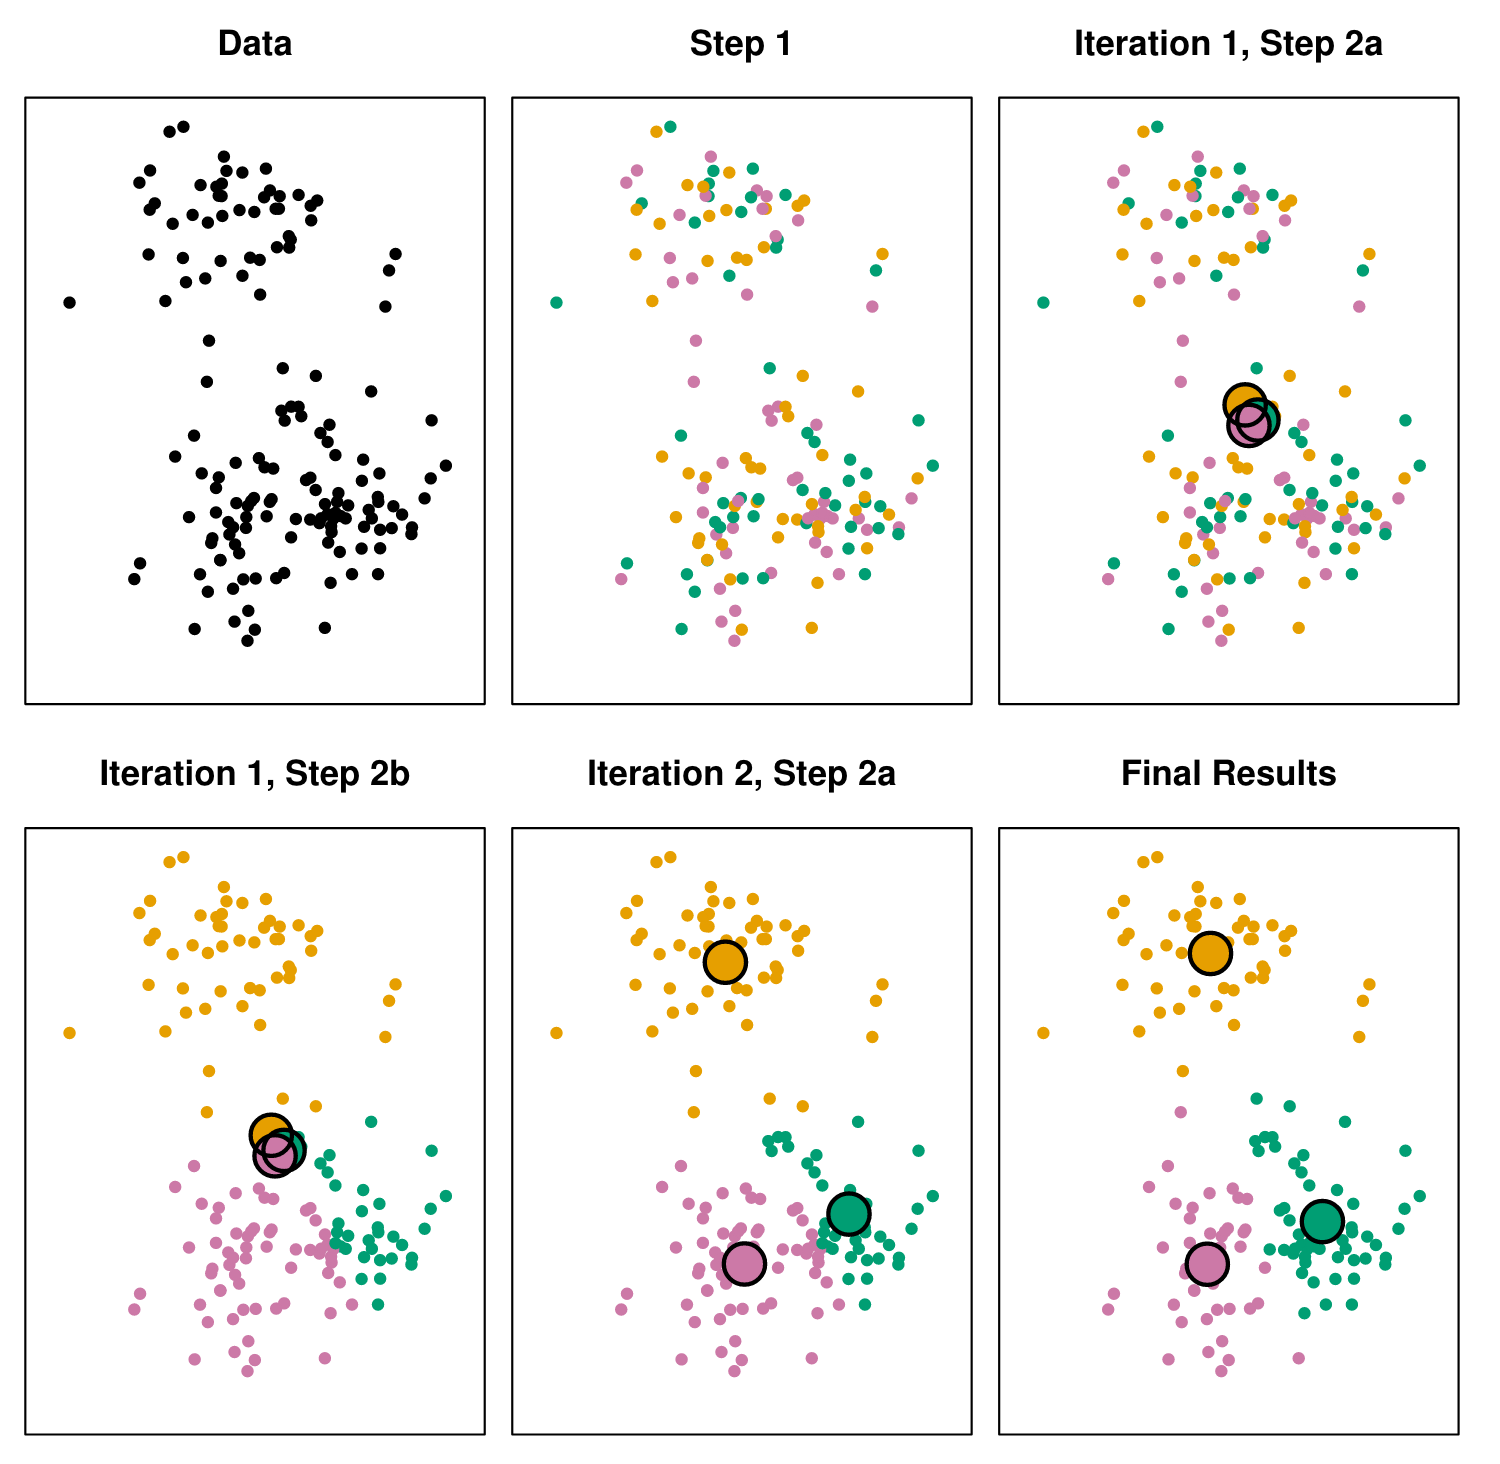
\includegraphics[width=0.7\textwidth]{Images/clustiteration.png}
    \caption[K-Means clustering iterations.]{The progress of the K-means algorithm with $K=3$. Adapted from \cite{james_introduction_2021}.}
    \label{fig:clustiteration}
\end{figure}
Because the K-means algorithm finds a local rather than a global optimum, the results obtained will depend on the initial (random) cluster assignment of each observation in Step 1 of Algorithm \ref{alg:kmeans}. In our case, as we will see shortly, this will not be an issue because, thanks to bagging clustering, the problem will not arise.
% <<< End of Unsupervised classification



% Functional Data Analysis >>>
\section{Functional Data Analysis}
\label{sec:fda}
\textbf{\textcolor{red}{To be completed.}}
\\
%In the Indeed, functional data analysis (FDA) is a branch of statistics that deals with data represented as functions. Instead of observing data at a set of fixed points, as is common in traditional statistics, FDA focuses on data that comes in the form of curves, surfaces, or even more general objects. Common examples include temperature or financial data over time. FDA provides tools and techniques to analyze and understand the intrinsic nature of such functional data. It allows for the examination of variability and dynamics within the data and can be particularly useful when understanding patterns or trends in the data is of importance. In our case, the 
In this section, I will discuss Functional Data Analysis (FDA) and Functional Principal Component Analysis (FPCA). Once again, I will provide a brief overview to give readers the foundational knowledge needed to understand the algorithm described in section \ref{sec:bvc}. 

\textit{Here a small introduction of FDA from \cite{ramsay_functional_2009}}
\subsection{Functional Principal Component Analysis}
% <<< End of Functional Data Analysis


% Bagging Voronoi Clustering Algorithm >>>
\section{Bagging Voronoi Classifier}
\label{sec:bvc}
Bagging Voronoi Clustering Algorithm is an algorithm presented in Secchi et al. \cite{secchi_bagging_2013} and it is an algorithm for unsupervised classification of functional data that exploits spatial dependence by repeatedly generating random connectivity maps and by clustering, at each replicate, local representatives of neighboring functional data. The algorithm is completely non-parametric, thus we don't need any apriori hypothesis on data distributions. With this algorithm, we should be able to spot regions in the printing plate with anomalous behaviour. Before detailing the steps of the algorithm, I believe it's useful to introduce a fundamental concepts: Voronoi tessellation. Voronoi diagram is a partition of a plane into regions close to each object of a given set. In our case, these objects are just the sites of the lattice $\mathcal{S}_0$. We call these objects nuclei. For each nucleus, there is a corresponding region, called a Voronoi cell, consisting of all points of the plane closer to that nucleus than to any other. Let's then provide a formal definition of a Voronoi cell. Let $X$ be a metric space and let $d(\cdot, \cdot)$ be a distance function, in our case Euclidean distance. Let $\Phi_n$ be the set of $n$ selected nuclei and let each nucleus be a tuple of coordinates $\left(P_k\right)_{k\in \Phi_n}$. The Voronoi cell $R_k$ associated with the site $P_k$ is defined as
\begin{equation}
    \label{eq:voronoicell}
    R_k=\{x\in X \mid d(x, P_k)\leq d(x, P_j),\forall j\neq k\}
\end{equation}
The Voronoi tessellation is simply the collection of all the cells in the space.
An example of a Voronoi tessellation can be seen in Fig. \ref{fig:voronoi}.
\begin{figure}[H]
    \centering
    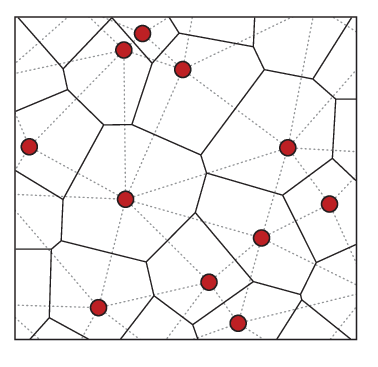
\includegraphics[width=0.4\textwidth]{Images/A-set-of-atoms-the-associated-Voronoi-tessellation-solid-lines-and-the-Delaunay.png}
    \caption[Voronoi tessellation.]{Example of Voronoi tessellation with highlighted nuclei.}
    \label{fig:voronoi}
\end{figure}


\subsection{Algorithm Steps}
\label{subsec:algsteps}
In this section, I will provide a detailed description of algorithm steps.
Suppose a latent field of labels $\Lambda_0:\mathcal{S}_0 \rightarrow \{1,\dots,L\}$ which is defined on the lattice $\mathcal{S}_0$. $\Lambda_0(\mathbf{x})$ is the true unknown label associated to the site $\mathbf{x}\in\mathcal{S}_0$, where $\mathcal{S}_0 \subset \mathcal{S}$ and $\mathcal{S}$ is a measurable subset of $\mathbb{R}^d$. In addition, suppose that a functional datum is observed in each site $\mathbf{x}\in\mathcal{S_0}$.
\paragraph{Step 1: Voronoi Tessellation} Select a set of points $\mathbf{x}\in\mathcal{S}$ as nuclei for the Voronoi tessellation. Thus, let $\Phi_n=\{\mathbf{Z}_1, \dots, \mathbf{Z}_n\}$ be a set of $n$ points in $\mathcal{S}$ sampled from a proper distribution $F$ defined on S: this will be the set of nuclei of the Voronoi tessellation. For each $\mathbf{Z}_i\in\Phi_n$ define the polyhedron
\begin{equation}
    \label{eq:polyedron}
    V\left(\mathbf{Z}_i \mid \Phi_n\right)=\{\mathbf{x}\in\mathcal{S} : d\left(\mathbf{x},\mathbf{Z}_i\right) \leq d\left(\mathbf{x}, \mathbf{Z}_j\right), \quad \text{for all}\quad \mathbf{Z}_j \in \Phi_n, i\neq j\}
\end{equation}
to be the closest Voronoi cell with nuclues $Z_j$ for the Voronoi tessellation induced by $\Phi_n$.
\paragraph{Step 2: Functional Local Representatives} Consider T, a bounded interval of $\mathbb{R}$ and a realization $f_{\mathbf{x}}:T\rightarrow \mathbb{R}$ of a functional random variable is observed in each site $\mathbf{x}$ of the lattice $S_0$. From the previous step, we got a Voronoi tessellation of the lattice $S_0$ which define random neighborhoods. For each element $V_i$ of the Voronoi tessellation, we sum up the information contained in the sub-sample $\{f_{\mathbf{x}}\}_{\mathbf{x} \in V_i}$ by estimating a functional local representative through a method that exploits spatial dependence of neighboring data. As example, the authors suggest to use weighted mean with a Gaussian kernel, but we can use any local representative we want. For $i=1, \dots, n$ the functional local representative $g_i$ aforementioned is defined as
\begin{equation}
    \label{eq:gaussianmean}
    g_i(t)=\frac{\sum_{\mathbf{x}\in V_i}w^i_{\mathbf{x}}\cdot f_{\mathbf{x}}(t)}{\sum_{\mathbf{x}\in V_i}w^i_{\mathbf{x}}}
\end{equation}
where $w_{\mathbf{x}}^i$ is a Gaussian weight centered in $Z_i$ and decreasing with respect to $d\left(\mathbf{x}, \mathbf{Z}_i\right)$. Intuitively we assume that spatial dependence between two sites decreases when the distance between them increases. The kernel covariance matrix is $\sigma^2\mathbb{I}_2$, where $\sigma=d_{max}/d_{min}$, being $d_{max}$ and $d_{min}$ the maximum and minimum distance between two nuclei of the tessellation, respectively. This choice connects $\sigma$ to the mean dimension of the tessellation element via an estimator of the elements mean diameter. The choice of $n$, which sets the tessellation dimension and thus the number of local representatives to be computed, has great influence on the algorithm behavior: in general, we have to find an optimal $n$ such that finds a good compromise between variance and bias.

\paragraph{Step 3: Dimensional Reduction and Clustering} To obtain the label for each site, we then perform k-mean clustering on the sample of the $p$-vectors of the scores $\{\mathbf{g}_1, \dots, \mathbf{g}_n\}$. Repeat steps 1-3 $B$ times, where $B$ is arbitrary chosen. 

\paragraph{Step 4: Cluster Matching} The output of the $b$-th replicate of the bootstrap phase of the algorithm is a label assignment for each local representative estimated during the $b$-th run. All sites $\mathbf{x}$ in $V_i^b$ get the same label associated to the function local representative $g_i^b(t)$. To obtain a classification map of the lattice $\mathcal{S}_0$, we consider the frequency distribution of assignment of each site to each of the $K$ clusters along the $B$ replicates. To compute this frequency distribution we need in turn to assume that cluster labels $\{C_1^b, \dots, C_K^b\}$ are coherent along the B replicates. More specifically, we want cluster labels $\{C_1^b, \dots, C_K^b\}$ to be coherent with $\{C_1^m\, \dots, C_K^m\}$, for all $m<b$ and $b\geq2$. This is obtained through cluster matching. Cluster matching is a set of techniques that allow us to keep different clustering algorithm outputs coherent. I will discuss a simple approach based on the use of contingency table. The algorithm looks for the label permutation that minimizes the total sum of the off-diagonal frequencies in the contingency table describing the joint distribution of sites along the classifications at two subsequent replicates. At the end of clustering matching, for each site $\mathbf{x}$ we will have a vector $\pi_{\mathbf{x}}^K=\left(P_1, \dots, P_K\right)$ where each $P_i, \quad i=1,\dots,k$ is the frequency the label $k$ was assigned to the site $\mathbf{x}$. The final label will be the label associated to maximum $P_k$. In other words, we it is a majority voting among the different replicates $b$.

\paragraph{Step 5: Evaluate Output} To have an overview of the statistical validity of the clustering just performed, we can use \textit{spatial entropy}. This concept is directly derived from the classical notion of entropy. Considering the frequency distribution vector $\boldsymbol{\pi}=(\pi_{\mathbf{x}}^1,\dots,\pi_{\mathbf{x}})^K$ of each site $\mathbf{x} \in \mathcal{S}_0$ to each of the $K$ clusters obtained after the bootstrapping step of the algorithm. The entropy associated to the final classification in the site $\mathbf{x}\in\mathcal{S}_0$ is defined as
\begin{equation}
\mathbf{\pi}_{\mathbf{x}}=-\sum_{k=1}^K\pi_{\mathbf{x}^k}\cdot \log(\pi_{\mathbf{x}^k})
\end{equation}
which assumes the minimum value 0 when there is an $r$ such that $\pi_{\mathbf{x}}^r=1$ while $\pi_{\mathbf{x}}^k=0$ for all $k\neq r$ and maximum value $\log(K)$ when $\pi_{\mathbf{x}}^k=\frac{1}{K}$ for $k\in\{1,\dots,K\}$. We can see spatial entropy as the degree of order of the frequency of assignment the site $\mathbf{x}\in\mathcal{S}_0$to cluster $k$. Moreover, we can compute the \textit{average normalized entropy} to have a global evaluation index of the clustering performed. Average normalized entropy is defined as
\begin{equation}
\label{eq:avgentropy}
    \eta^K=\frac{\sum_{\textbf{x}\in\mathcal{S}_0}\eta_{\mathbf{x}}^K}{\log(K)\cdot |\mathcal{S}_0|}
\end{equation}
From \ref{eq:avgentropy} we can appreciate how the index hsa been normalized to maximum value $\log(K)$ in order to allow comparison over different choices of $K$. An other possible index for evaluating a classification in the ratio
\begin{equation}
    \label{eq:theta}
    \theta=\frac{tr(B)}{tr(B)+tr(W)}
\end{equation}
where $B$ and $W$ are the final between and within cluster sum of squares matrix, respectively. This index can be seen as the percentage of variance explained by splitting the observations in clusters.

\begin{algorithm}[H]
    \caption{Bagging Voronoi Classifiers}
    \label{alg:bvc}
    \begin{algorithmic}[1]
    \STATE \textbf{Bootstrap:}
    \STATE Initialize $B, n, p, K$. Choose a metric $d(\cdot,\cdot).$
    \FOR{$b:=1$ to $B$}
    \STATE{Randomly generate a set of nuclei $\Phi^b_n=\{\mathbf{Z}_1^b, \dots, \mathbf{Z}_n^b\}$ among the sites in $\mathcal{S}_0$}
    \FOR{$i=1$ to $n$}
    \STATE $\mathbf{Z}_i^b\sim\mathcal{U}(\mathcal{S}_0)$, where $\mathcal{U}$ is the uniform distribution on the lattice. Obtain a random Voronoi tessellation of $\mathcal{S}_0, \{V(\mathbf{Z}_i^b|\Phi_n^b\}^n_{i=1}$ by assigning each site $\mathbf{x}\in \mathcal{S}_0$ to the nearest nucleus $\mathbf{Z}_i^b$, according to the specified distance $d(\cdot,\cdot).$
    \ENDFOR
    \FOR {$i:=1$ to $n$}
    \STATE Compute the function $g_i^b$, acting as local representative, by summarizing information carried by the functional data associated to sites belonging to the $i$-th element of the tessellation $V(\mathbf{Z}_i^b|\Phi_n^b)$.
    \ENDFOR
    \STATE Perform dimensional reduction of the local representatives $\{g_1^b,\dots, g_n^b\}$ by projecting them on the space spanned by a proper $p$-dimensional scores vectors $\{\mathbf{g}_1^b,\dots, \mathbf{g}_n^b\}$, which are then clustered in $K$ groups according to suitable unsupervised method.
    \ENDFOR
    \STATE \textbf{Aggregation:} perform cluster matching
    \FOR {$k:=1$ to $K$}
    \FOR {$b:=1$ to $B$}
    \STATE indicate with $C_k^b$ the set of $\mathbf{x} \in \mathcal{S}_0$ whose label is equal to $k$, and match the cluster labels across bootstrap replicates, to ensure identifiability.
    \ENDFOR
    \ENDFOR
    \FOR {$\mathbf{x} \in \mathcal{S}_0$}
    \STATE Calculate the frequencies of assignment of the site to each of the $K$ clusters along iterations, \textit{i.e.}, $\pi_{\mathbf{x}}^k=\#\{b\in\{1,\dots,B\}:\mathbf{x}\in C_k^b\}/B, \forall k=1,\dots,K$
    \ENDFOR
    \end{algorithmic}
\end{algorithm} 

% <<< End of Bagging Voronoi Clustering Algorithm

% Succesful case of the algorithm >>>
\section{Successful Case Studies in Clustering Algorithm Application}
\label{sec:bcv-cases}
In this section, we will discuss two examples of how the algorithm outlined in the previous section has been successfully applied in two completely different domains: the clustering of irradiance data performed in \citeauthor{secchi_bagging_2013} \citeyear{secchi_bagging_2013} and the analysis of spatio-temporal mobile phone data performed in \citeauthor{secchi_analysis_2015} \citeyear{secchi_analysis_2015}. The purpose of this section is to address any potential questions or uncertainties the reader may still have regarding the use of the algorithm detailed Section \ref{sec:bvc}.

\subsection{Clustering of Irradiance Data}
\label{subsec:irradiance}
Insolation refers to the amount of solar radiation energy captured on a specific surface area over a set duration. Typically, it is denoted as average irradiance in kilowatt-hours per square meter per day (\unit{\kilo\watt.h/\metre^2.day}). Authors focused on direct insolation, which pertains to the solar irradiance measured at a particular location on Earth with a surface facing directly towards the sun's rays, omitting diffuse insolation. Diffuse insolation refers to the solar energy scattered or reflected by atmospheric components overhead. The value of direct insolation is derived from the solar constant minus the atmospheric reductions from absorption and scattering. While the solar constant is influenced by factors like Earth's distance from the sun and solar cycles, the losses are contingent on factors such as the time of day (which affects the light's path through the atmosphere based on the sun's elevation angle), cloud coverage, atmospheric moisture, and other contaminants. Author's goal was to identify areas of the planet which are optimal with respect to the positioning of solar power collectors by considering parameters, which depend on direct insolation. The data available for the analysis consists of vectors in $\mathbb{R}^{12}$ indexed by each site of the lattice. Sites are located on a non-uniform lattice $\mathcal{S}_0=\bigcup_{\lambda \in Z_{\mathbf{1}};\theta \in Z_{\mathbf{2}}}A_{\lambda\theta}$ where $Z_{\mathbf{1}} = \{ -180, -179, \dots, 178, 179\}$ and $Z_{\mathbf{2}} = \{ -66, -65, \dots, 65\}$: each element $A_{\lambda\theta}$ is the portion of the earth surface which is included between the meridians at longitude $\lambda$ and $\lambda + 1$ in degrees, and between the parallels at latitude $\theta$ and $\theta + 1$ in degrees. This lattice is of course non-uniform, and includes 47,520 worldwide non-polar districts. In each site, the 12 measures correspond to the values of the monthly maximum energy deficit with respect to the monthly average. Both the maximum and the average values are computed over the 22 years time period from July 1983 to June 2005. For each site, they obtained a functional datum $Y_{\lambda,\theta}(t)$ by smoothing $\{Y_{\lambda\theta}^1, \dots, Y_{\lambda\theta}^12\}$ with a Gaussian kernel with bandwidth equal to 1.5, where $Y_{\lambda\theta}^\nu$ is the irradiance data for each month. The authors chose to use a Gaussian isotropic kernel to compute the local representatives. They selected the first $p=3$ functional principal components since only with these was the proportion of explained variance greater than 95\%. For classifying the scores of the $n$ representatives, they employed the K-Means algorithm described in Section \ref{subsec:kmeans} with the $L^2$ semi-metric induced by the principal components.

\begin{figure}[H]
    \centering
    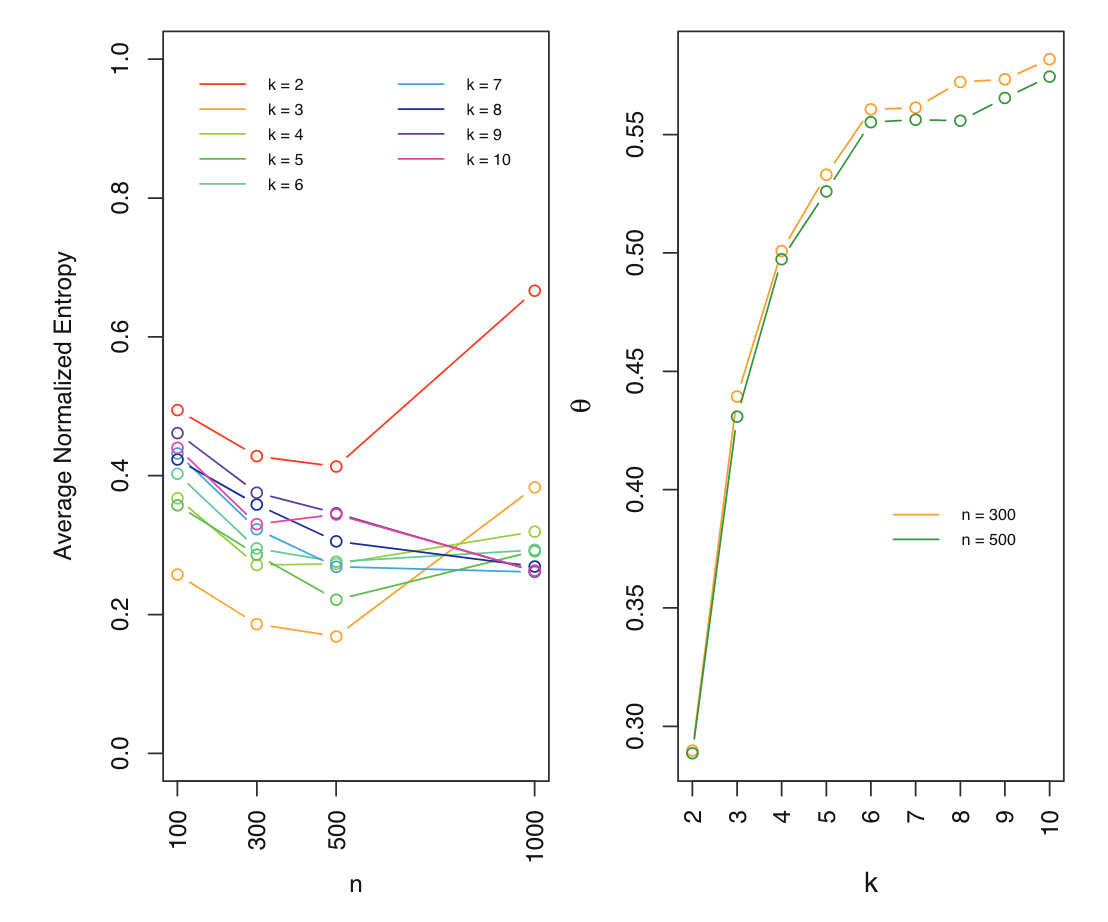
\includegraphics[scale=0.5]{Images/baggingscreeplot.png}
    \caption[Result on irradiance data.]{Algorithm performances with irradiance data. On the left, average normalized entropy, on the right the index $\theta$. From \citeauthor{secchi_bagging_2013} \citeyear{secchi_bagging_2013}.}
    \label{fig:baggingscreeplot}
\end{figure}
Subsequently, as with all classical clustering problems, they performed the clustering multiple times in order to obtain the scree-plot shown in Fig. \ref{fig:baggingscreeplot} and to select the optimal number of clusters, $K$. Additionally, with this specific algorithm, it was also necessary to determine the optimal number of nuclei, $n$, for the initial Voronoi tessellation, as detailed in Algorithm \ref{alg:bvc}. To find the scree-plots shown in the above figure, the number of bootstrap replications was set at $b=100$, and the parameters $n$ and $K$ were varied. The optimal choice for these two parameters was made by using average normalized spatial entropy, the index $\theta$, and the normalized spatial entropy map in conjunction. Starting from the scree-plot of average normalized entropy in Fig. \ref{fig:baggingscreeplot}, we can see that for $n=500$, we have two local minima, specifically for $K=3$ and $K=5$. From the above figure, we can observe that the graph of the t-index suggests that the number of clusters $K=6$ appears to be the most reasonable. Indeed, using $K=7$ would not be sensible as it would not enhance the classification obtained. Consequently, the classification should yield good results for $K=5$ and $K=6$. This was also confirmed by the maps of the normalized entropy, shown in Fig. \ref{fig:irrentropy}.

\begin{figure}[H]
    \centering
    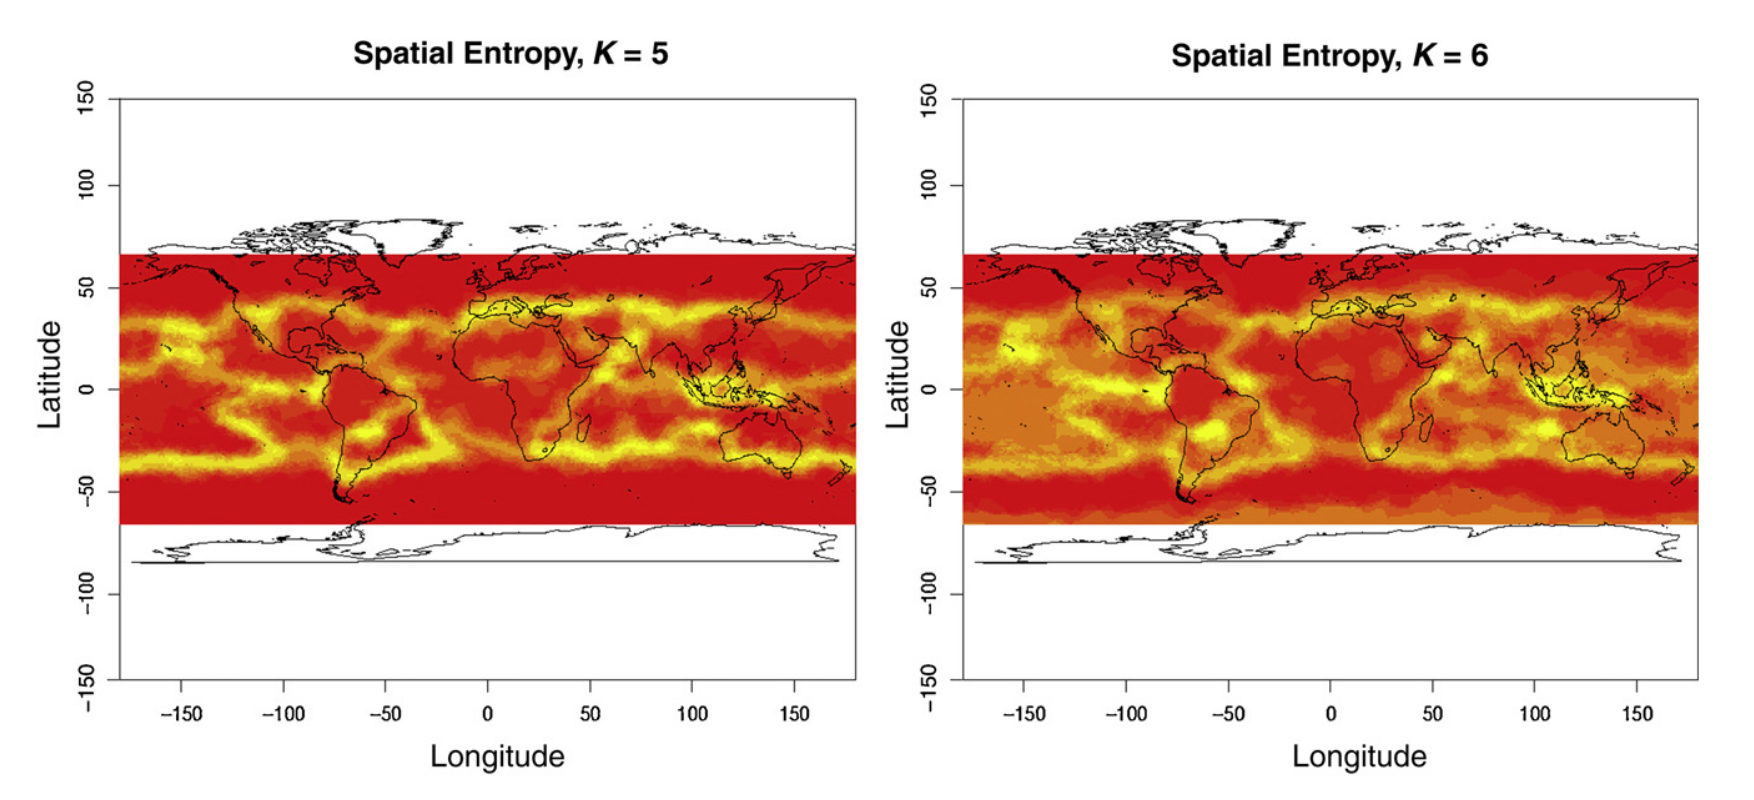
\includegraphics[scale=0.5]{Images/irrentropy.png}
    \caption[Spatial entropy for irradiance data.]{Normalized spatial entropy maps associated to the classification with K = 5 (left) and K = 6 (right). Colors from red to white correspond to values from 0 to 1; higher values identify areas where classification is more uncertain. From \citeauthor{secchi_bagging_2013} \citeyear{secchi_bagging_2013}.}
    \label{fig:irrentropy}
\end{figure}

The final choice $K=5$ was made looking at maps in Fig. \ref{fig:irrentropy}, which tell us that for $K=5$ the classification is more robust, and from the fact that with $K=5$, the algorithm identified different homogeneous macro-areas which seem interpretable in terms of observed phenomenon. In Fig. \ref{fig:resbagging} there are the final cassifications for irradiance data. Now, as mentioned earlier, we can take advantage of the functional nature of the data to derive additional insights that wouldn't be possible with traditional clustering algorithms. For instance, the fact that the red cluster exhibits a non-seasonal pattern that remains consistent throughout the year, or how the green and yellow clusters have opposite seasonal patterns. Lastly, it's noteworthy to observe that spatial entropy is systematically higher near the boundary between two clusters. This is due to the fact that the functional data is spatially dependent, and hence data near the boundaries are more challenging to cluster.

\begin{figure}
    \centering
    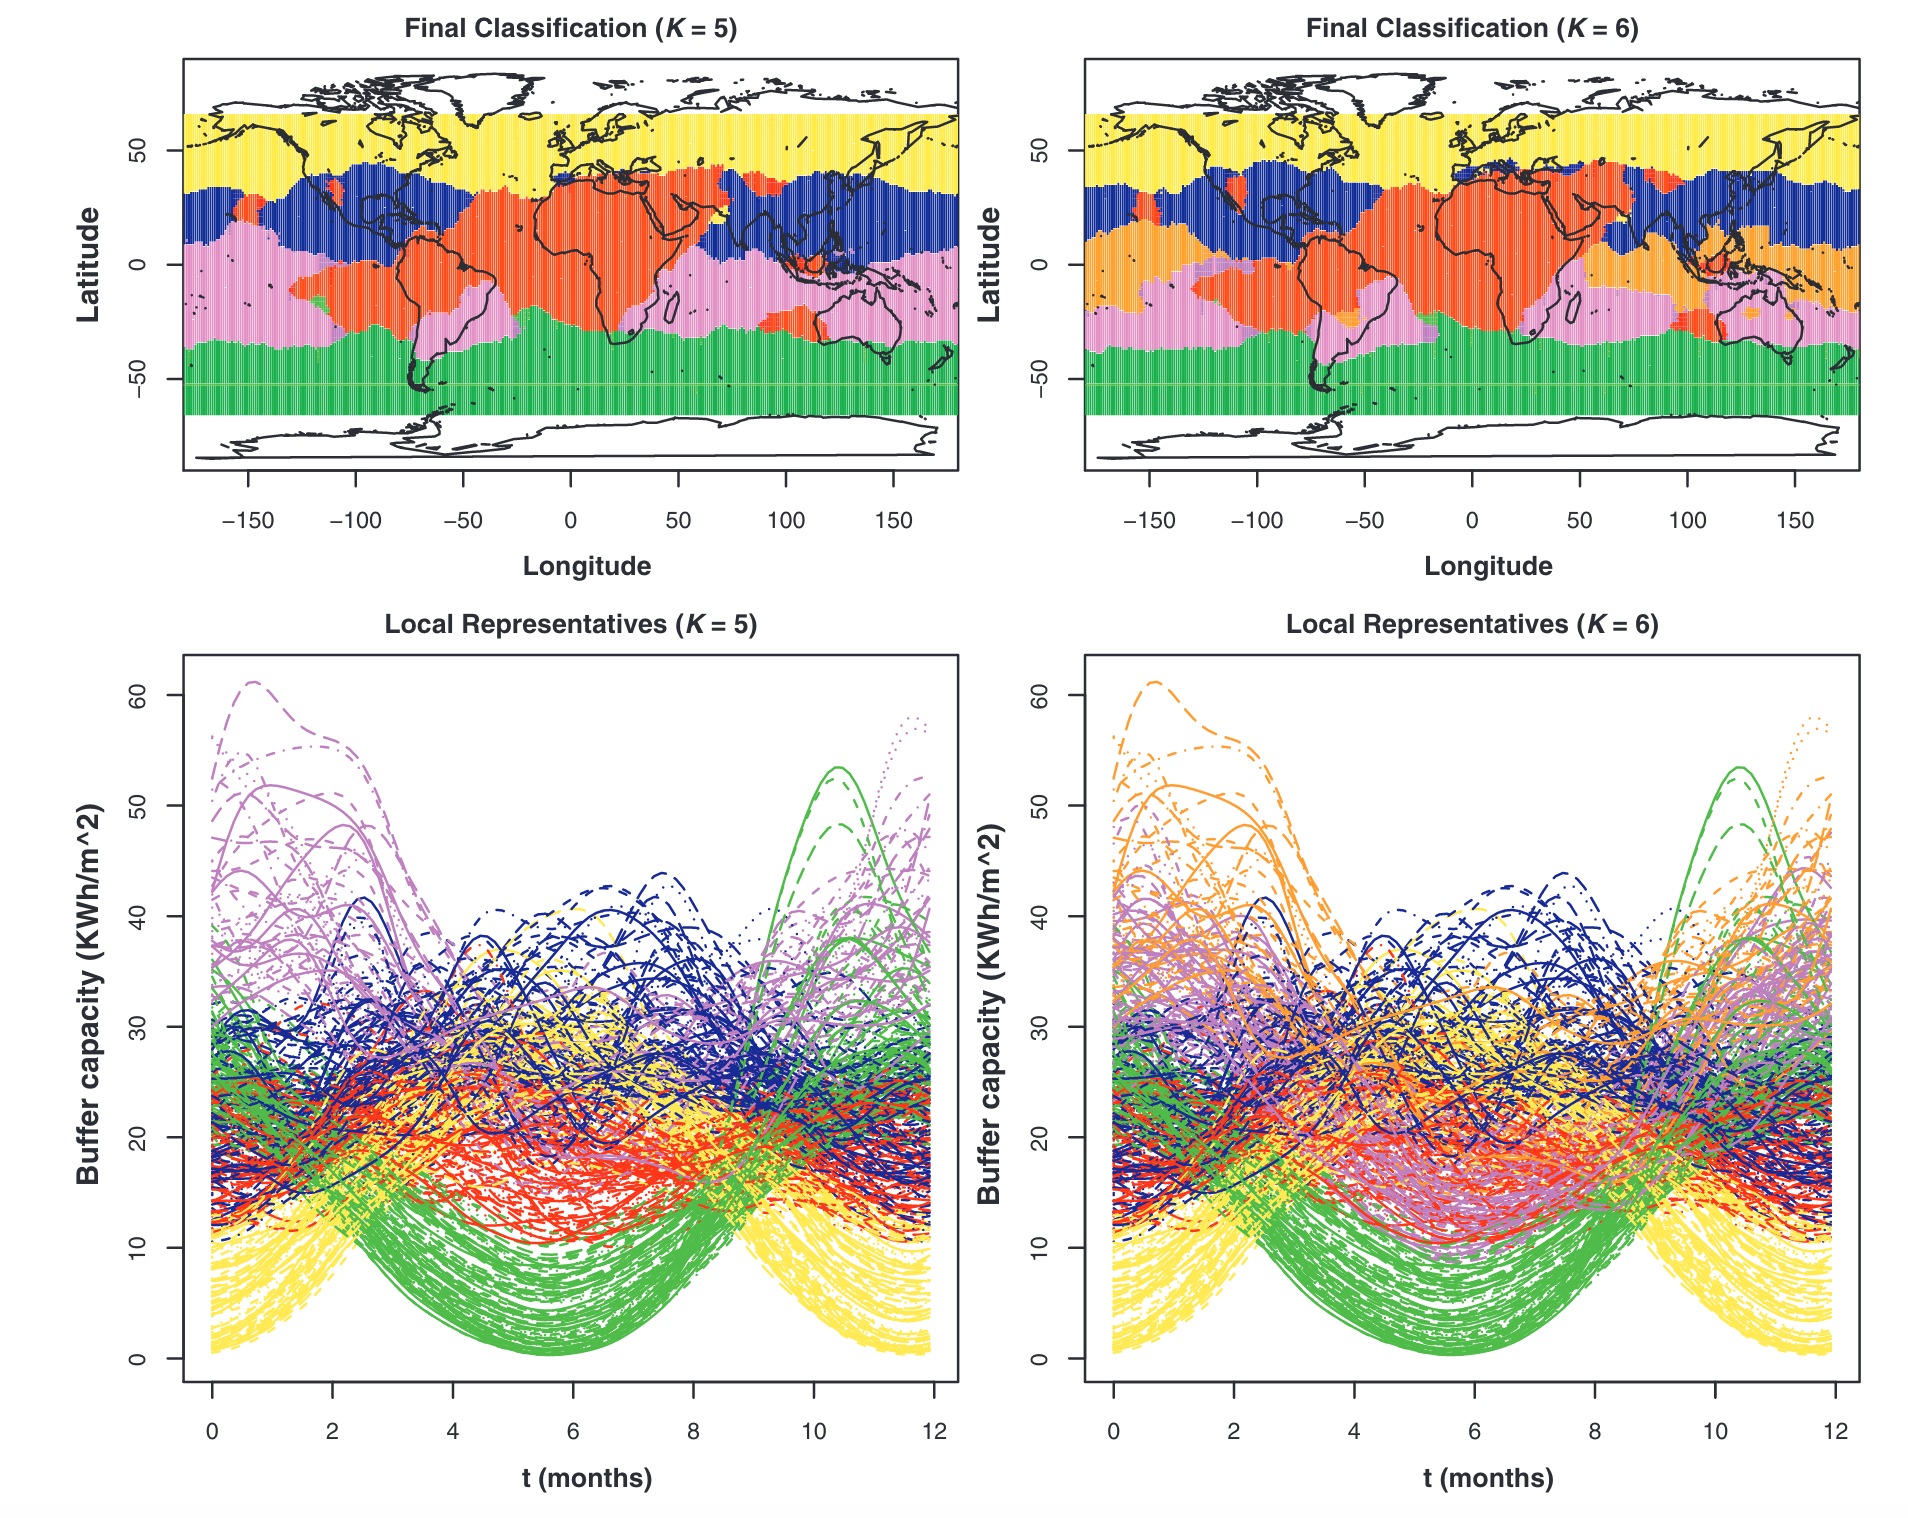
\includegraphics[scale=0.4]{Images/resbagging.png}
    \caption[Classification of irradiance data.]{In the top panels, final classification maps obtained via a majority vote on frequencies of assignment, and by setting $K = 5$ (left) or $K = 6$ (right).In the bottom panels, a set of functional local representatives obtained with $n = 500$ in one of the iterations of the algorithm and clustered with $K = 5$ (left) and with $K=6$ (right). From \citeauthor{secchi_bagging_2013} \citeyear{secchi_bagging_2013}.}
    \label{fig:resbagging}
\end{figure}






\subsection{Analysis of Spatio-Temporal Mobile Phone Data in Milan}
\label{subsec:mobilephonemilan}
% <<< End of Succesful case of the algorithm